\documentclass[11pt]{article}
\usepackage[margin=1in]{geometry}
\usepackage[T1]{fontenc}
\usepackage{lmodern}
\usepackage{graphicx}
\usepackage{booktabs}
\usepackage{amsmath,amssymb}
\usepackage{tikz}
\usetikzlibrary{positioning,arrows.meta,shapes.geometric,fit,backgrounds}
\usepackage{xcolor}
\usepackage{caption}
\usepackage{microtype}
\usepackage[hidelinks]{hyperref}
\usepackage{array}
\usepackage{enumitem}
\setlist{itemsep=2pt,topsep=3pt}
\captionsetup{font=small,labelfont=bf}

\definecolor{cblue}{HTML}{2A78D6}
\definecolor{corange}{HTML}{EB6834}
\definecolor{cgray}{HTML}{8A8985}

\title{Glaucoma Detection by Combining SLO and OCT Fundus Images:\\
A Systematic Comparison of CNN, Transformer and Hybrid Models}
\author{Rushikesh}
\date{November 2026}

\begin{document}
\maketitle

%==============================================================================
\section{Introduction}
Glaucoma is a progressive optic neuropathy and a leading cause of irreversible blindness. Vision lost to glaucoma
cannot be restored, so detecting the disease early matters, and automated screening from retinal imaging is an
attractive way to scale detection. Two imaging modalities are routinely acquired in the clinic: scanning laser
ophthalmoscopy (SLO) fundus images, which show the surface of the retina, and optical coherence tomography (OCT),
which captures retinal structure, including the nerve-fibre layer, in depth. The two views are complementary, so a
model that sees both should in principle detect glaucoma better than a model that sees only one.

In this project we solve a specific problem: \emph{binary glaucoma classification from a pair of images of the same
eye, an SLO fundus image and an OCT-derived fundus image}, on the FairDomain data~\cite{fairdomain}. The data
also carry demographic attributes (gender, race, ethnicity), because the dataset was built to study algorithmic fairness; we therefore report
performance not only overall but also per demographic group.

The project has three goals. (i)~Establish how well standard deep architectures solve the task, and in particular how much
(a) ImageNet pretraining, (b) fusing the two modalities, and (c) the choice of architecture family (CNN,
transformer, hybrid) matter. (ii)~Find out which training choices are worth their cost on a small dataset
(2{,}550 training images after holding out validation data), where overfitting is the dominant difficulty. (iii)~Check
whether common fairness interventions and ensembling change the picture. Because the test set is small
(2{,}000 images), we pay particular attention to statistical uncertainty and avoid ranking models whose differences lie
within it.

\paragraph{Contributions.}
(1)~A controlled comparison of CNN, transformer and hybrid backbones and several fusion strategies (more than 50 training runs in three sweeps) on SLO+OCT glaucoma
classification, with bootstrap confidence intervals and per-group metrics.
(2)~An ablation study of the training recipe that corrects one of our own hypotheses (Section~\ref{sec:abl}).
(3)~Evidence that, at this data scale, averaging several models is the most reliable gain, whereas architecture choice and
fairness-specific losses are not distinguishable from noise.

%==============================================================================
\section{Related Work}
\paragraph{Fairness-oriented ophthalmic datasets.}
The Harvard Ophthalmology AI Lab released a series of datasets pairing retinal imaging with demographic
attributes. Harvard Glaucoma Fairness~\cite{harvardgf} introduced a glaucoma dataset with 2D and 3D
imaging and proposed Fair Identity Normalization (FIN), which equalises feature importance across identity groups.
Harvard Eye Fairness~\cite{harvardeye} extended this to 30{,}000 subjects with 3D OCT and proposed Fair Identity Scaling
(FIS), a loss weighting that combines individual and group scaling. FairCLIP~\cite{fairclip} studies fairness in
vision--language learning on related data. FairDomain~\cite{fairdomain}, whose data we use, studies fairness under
\emph{domain shift} for both segmentation and classification, treating different image types as domains, and proposes
a fair identity attention (FIA) module. Group-wise AUC, worst-group AUC and equity-scaled AUC (ES-AUC) are the fairness-aware metrics commonly reported in this line of work.

\paragraph{Recent glaucoma-specific work.}
FairEnc~\cite{fairenc} builds a fair vision--language model on SLO images paired with clinical notes, Fair-Eye
Net~\cite{faireyenet} combines fundus photographs, OCT-derived metrics and visual-field indices with a fairness constraint, and
RED-Sphere~\cite{redsphere} targets cross-population domain generalisation for fundus disease. We did not
reproduce these methods; they motivate our use of per-group evaluation and of the two image types as separate domains.

\paragraph{Backbones and training techniques.}
We compare residual networks~\cite{resnet}, EfficientNet~\cite{efficientnet}, DenseNet~\cite{densenet}, RegNet~\cite{regnet} and
ConvNeXt~\cite{convnext} (convolutional); ViT~\cite{vit}, DeiT~\cite{deit} and Swin~\cite{swin} (transformers); and
CoAtNet~\cite{coatnet} and MaxViT~\cite{maxvit} (convolution--attention hybrids), plus a self-supervised DINOv2 ViT~\cite{dinov2}.
Pretrained weights are the default \texttt{timm} checkpoints~\cite{timm}: ImageNet-1k~\cite{imagenet} for most models, ImageNet-21k$\to$1k for ViT-Small, ImageNet-12k$\to$1k for ConvNeXt-Tiny, and the self-supervised LVD-142M data for DINOv2. The regularisers we study
are mixup~\cite{mixup}, CutMix~\cite{cutmix}, stochastic depth (drop-path)~\cite{stochdepth}, label smoothing~\cite{labelsmooth} and
weight averaging (EMA). For adversarial debiasing we use a gradient-reversal layer~\cite{grl}.

%==============================================================================
\section{Method}
\subsection{Problem formulation}
Each sample is a pair $(\mathbf{x}_S,\mathbf{x}_O)$ of $224\times224$ single-channel images (SLO fundus and OCT fundus),
a binary label $y\in\{0,1\}$ (glaucoma), and demographic attributes $g$ (used only for evaluation, except in the
fairness experiments). We learn $p(y=1\mid \mathbf{x}_S,\mathbf{x}_O)$.

\subsection{Architecture}
Figure~\ref{fig:arch} shows our main model. Each modality is processed by its own backbone
($f_S$, $f_O$, same architecture, separate weights, initialised from ImageNet), producing feature vectors
$\mathbf{z}_S,\mathbf{z}_O$. The fusion module combines them and a dropout--linear head outputs the glaucoma logits.
We study these fusion variants:
\begin{itemize}
\item \textbf{Late fusion (default):} $\mathbf{z}=[\mathbf{z}_S;\mathbf{z}_O]$.
\item \textbf{Early fusion:} one backbone receives the two images as a 2-channel input.
\item \textbf{Gated fusion:} $\mathbf{z}=\sigma(W[\mathbf{p}_S;\mathbf{p}_O])\odot \mathbf{p}_S+(1-\sigma(\cdot))\odot \mathbf{p}_O$ with projections
$\mathbf{p}=W'\mathbf{z}$, trained with modality dropout (one modality's feature is zeroed for 20\% of samples).
\item \textbf{Cross-attention fusion} (ViT-Small only): the token sequence of each modality attends to the other's tokens
before the class tokens are concatenated.
\item \textbf{Single modality:} one backbone sees only SLO or only OCT (an ablation).
\end{itemize}
Pretrained first-layer filters are adapted to one input channel by \texttt{timm} (summing the RGB filters).
Pixels are scaled to $[0,1]$ and normalised as $(x-0.5)/0.25$.

\begin{figure}[t]
\centering
\resizebox{\linewidth}{!}{%
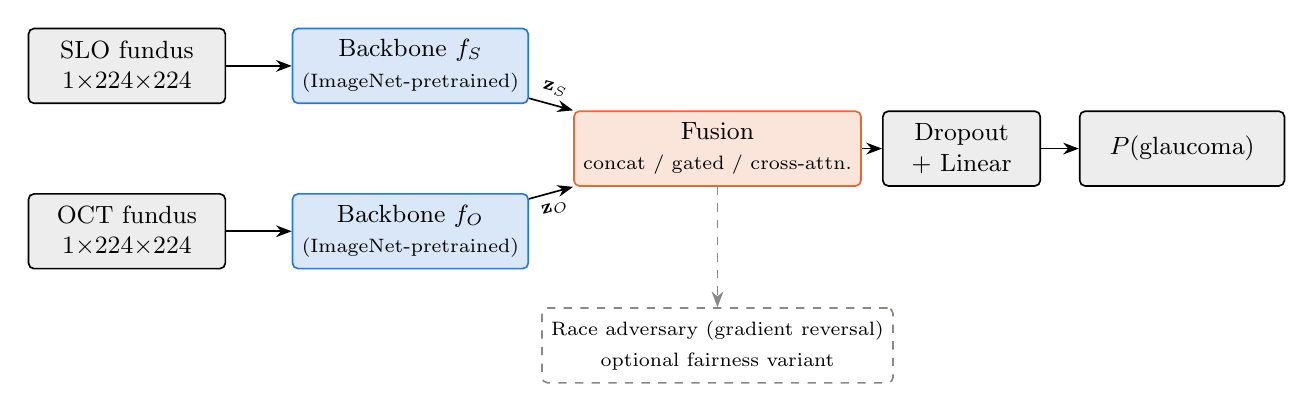
\begin{tikzpicture}[
  box/.style={draw,rounded corners=2pt,minimum height=0.95cm,align=center,font=\small,line width=0.6pt},
  inp/.style={box,fill=cgray!15,minimum width=2.5cm},
  bb/.style={box,fill=cblue!18,draw=cblue,minimum width=2.7cm},
  fus/.style={box,fill=corange!18,draw=corange,minimum width=3cm},
  hd/.style={box,fill=cgray!15,minimum width=2cm},
  outb/.style={box,fill=cgray!15,minimum width=2.6cm},
  arr/.style={-{Stealth[length=2mm]},line width=0.6pt}]
\node[inp] (slo) at (0,1.05) {SLO fundus\\ $1{\times}224{\times}224$};
\node[inp] (oct) at (0,-1.05) {OCT fundus\\ $1{\times}224{\times}224$};
\node[bb] (fs) at (3.6,1.05) {Backbone $f_S$\\ \scriptsize (ImageNet-pretrained)};
\node[bb] (fo) at (3.6,-1.05) {Backbone $f_O$\\ \scriptsize (ImageNet-pretrained)};
\node[fus] (fu) at (7.5,0) {Fusion\\ \scriptsize concat / gated / cross-attn.};
\node[hd] (hd) at (10.6,0) {Dropout\\ + Linear};
\node[outb] (ou) at (13.4,0) {$P(\text{glaucoma})$};
\draw[arr] (slo) -- (fs);
\draw[arr] (oct) -- (fo);
\draw[arr] (fs) -- node[above,sloped,font=\scriptsize]{$\mathbf z_S$} (fu.north west);
\draw[arr] (fo) -- node[below,sloped,font=\scriptsize]{$\mathbf z_O$} (fu.south west);
\draw[arr] (fu) -- (hd);
\draw[arr] (hd) -- (ou);
\node[box,dashed,draw=cgray,minimum width=3.4cm] (adv) at (7.5,-2.5) {\scriptsize Race adversary (gradient reversal)\\ \scriptsize optional fairness variant};
\draw[arr,dashed,draw=cgray] (fu) -- (adv);
\end{tikzpicture}}
\caption{Two-branch late-fusion network. Each modality has its own backbone; the pooled features are fused and classified.
Variants replace the fusion block (gated, cross-attention), feed both images to a single backbone as two channels (early fusion),
use one branch only (single modality), or add an adversarial race head on the fused feature.}
\label{fig:arch}
\end{figure}

\subsection{Training recipe}
Our default \emph{plain} recipe (first sweep) uses cross-entropy, AdamW~\cite{adamw} with a one-cycle learning-rate
schedule~\cite{onecycle}, gradient clipping at 1.0, 15 epochs, horizontal flips and mild brightness jitter. The
\emph{stronger} recipe (later sweeps) adds, on the GPU: random rotation ($\pm15^\circ$), scaling ($\pm10\%$) and translation (up to 5\% of the image size);
label smoothing 0.1; an exponential moving average (EMA) of the weights (decay 0.995) used for evaluation; a $5\times$ learning rate on the new
head; and 25 epochs. Variants add mixup/CutMix, drop-path with rate 0.2 and head dropout 0.5, or a lower learning rate.
The epoch with the best validation AUC is kept.

\subsection{Fairness and domain-shift variants}
\begin{itemize}
\item \textbf{Group-reweighted loss:} each sample is weighted by the inverse frequency of its (race, label) cell.
\item \textbf{FIS-like loss:} per-sample weights equal to the product of the individual loss (relative to the batch mean) and its race group's mean loss
(relative to the batch mean), clipped to $[0.2,5]$ and renormalised. This is our approximation of the idea behind Fair Identity Scaling~\cite{harvardeye}, not an exact reimplementation.
\item \textbf{Adversarial debiasing:} a small classifier predicts race from the fused feature through a gradient-reversal layer~\cite{grl}
(loss weight 0.5, reversal strength ramped up during training).
\item \textbf{Cross-domain transfer:} one backbone is trained on one modality only and tested on the other (SLO$\to$OCT and OCT$\to$SLO), with the
unseen modality fed through the same single-channel input.
\end{itemize}

\subsection{Ensembling and test-time augmentation}
Ensembles average the predicted probabilities of several trained models. Test-time augmentation (TTA) averages a model's prediction on an image and on its horizontal flip.
Ensemble members in each experiment are chosen on validation AUC or fixed in advance (e.g.\ all five folds), never on test AUC.

%==============================================================================
\section{Experiments}
\subsection{Data}
We use the FairDomain release provided for this task: 5{,}000 samples (3{,}000 training, 2{,}000 testing), each stored as a
\texttt{.npz} file with an SLO fundus image, an OCT fundus image (both $224\times224$, 8-bit), the label, and demographic and clinical
attributes (age, gender, race, ethnicity, language, marital status, mean deviation MD). Segmentation masks are not included, so the task is classification.
Table~\ref{tab:data} summarises the splits. The groups are strongly imbalanced (73\% female, 77\% white, 4\% Hispanic), which matters for per-group evaluation.
From the 3{,}000 training images we hold out a stratified 15\% (450 images) as a \emph{validation} set used for early-stopping-style model selection and for all
automatic hyper-parameter decisions; models are trained on the remaining 2{,}550 images. The 2{,}000 test images are never used for training or for automatic selection.

\begin{table}[t]
\centering\small
\resizebox{\linewidth}{!}{\begin{tabular}{lrrrrrrr}
\toprule
 Split & $N$ & Glaucoma & Female & White & Black & Asian & Hispanic \\
\midrule
Training & 3000 & 1317 (44\%) & 2204 (73\%) & 2308 (77\%) & 467 (16\%) & 225 (8\%) & 121 (4\%) \\
Testing & 2000 & 887 (44\%) & 1449 (72\%) & 1522 (76\%) & 301 (15\%) & 177 (9\%) & 83 (4\%) \\
\bottomrule
\end{tabular}
}
\caption{Dataset composition. Percentages are of each split.}
\label{tab:data}
\end{table}

\subsection{Implementation and hyper-parameters}
All models are implemented in PyTorch~\cite{pytorch} with \texttt{timm}~\cite{timm} and trained in fp32 on a single Tesla P100 (16\,GB). Per-backbone learning rates, batch
sizes and weight decay (chosen once from common defaults for each family, without tuning) are in Table~\ref{tab:hp}; the stronger recipe in later sweeps
used EfficientNet-B0 with learning rate $5\times10^{-4}$, batch size 32 and weight decay $10^{-2}$ (head learning rate $\times5$) unless stated.
Sweep~1 trains for 15 epochs, later sweeps for 25 (one 12-epoch variant, and 15 epochs for the approximate sweep-1 re-run).
Model selection by validation AUC; seed 0 unless stated.

\begin{table}[t]
\centering\small
\begin{tabular}{lrrr}
\toprule
Backbone & Peak LR & Batch size & Weight decay \\
\midrule
ResNet18 (scratch) & 3e-4 & 64 & 1e-2 \\
ResNet50 & 2e-4 & 32 & 1e-2 \\
EfficientNet-B0 & 5e-4 & 32 & 1e-2 \\
DenseNet121 & 2e-4 & 32 & 1e-2 \\
ConvNeXt-Tiny & 1e-4 & 32 & 5e-2 \\
ViT-S / DeiT-S / Swin-T & 5e-5 & 32 & 5e-2 \\
CoAtNet-0 & 1e-4 & 32 & 5e-2 \\
MaxViT-Tiny & 5e-5 & 16 & 5e-2 \\
\bottomrule
\end{tabular}

\caption{Hyper-parameters of the first sweep (AdamW, one-cycle schedule, 15 epochs).}
\label{tab:hp}
\end{table}

\subsection{Evaluation protocol}
The main metric is the area under the ROC curve (AUC) on the 2{,}000 test images, which is threshold-free and insensitive to the 44/56 class balance. We also report accuracy at threshold 0.5.
To judge uncertainty we report non-parametric bootstrap 95\% confidence intervals over test images (300 resamples for per-run tables, 1{,}000 for ensembles and Figure~\ref{fig:overview}). Intervals are about $\pm0.02$ wide, so
differences smaller than that between two runs are not meaningful. Where it matters we use three seeds to measure training noise.
For fairness we report AUC within each gender, race and ethnicity group, the \emph{worst-group AUC} (minimum over gender and race groups with at least 100 test samples),
and the equity-scaled AUC (ES-AUC)
\begin{equation}
\text{ES-AUC}=\frac{\text{AUC}}{1+\sum_{g}\left|\text{AUC}-\text{AUC}_g\right|},
\end{equation}
computed separately per attribute (our implementation of the equity-scaled AUC used in the Harvard fairness benchmarks; absolute values may differ from the original definition).

\subsection{Baselines}
The reference baseline is a ResNet18 trained from scratch with the two-branch late-fusion design. The main comparison set is: pretrained ResNet50 (late and early fusion), EfficientNet-B0, DenseNet121, ConvNeXt-Tiny
(CNN-type); ViT-Small, DeiT-Small, Swin-Tiny (transformers); CoAtNet-0 and MaxViT-Tiny (hybrids); and EfficientNet-B0 on SLO only or OCT only (single-modality baselines).

\subsection{Results}
\paragraph{Overall comparison.}
Figure~\ref{fig:overview} and Table~\ref{tab:sweep1} (appendix) summarise the results. The from-scratch ResNet18 reaches 0.717 test AUC. Every pretrained model improves on it
(0.747--0.827). EfficientNet-B0 is the best single model in the first sweep (0.827), followed by Swin-Tiny (0.807) and DenseNet121 (0.803); the transformer and hybrid models are in the same
range as the CNNs (ViT-S 0.790, CoAtNet-0 0.793), and ConvNeXt-Tiny and ResNet50 are lower (0.767--0.768). Because the confidence intervals overlap almost entirely among the models between 0.79 and 0.83, we do not claim
a winner among architecture families.

\begin{figure}[t]
\centering
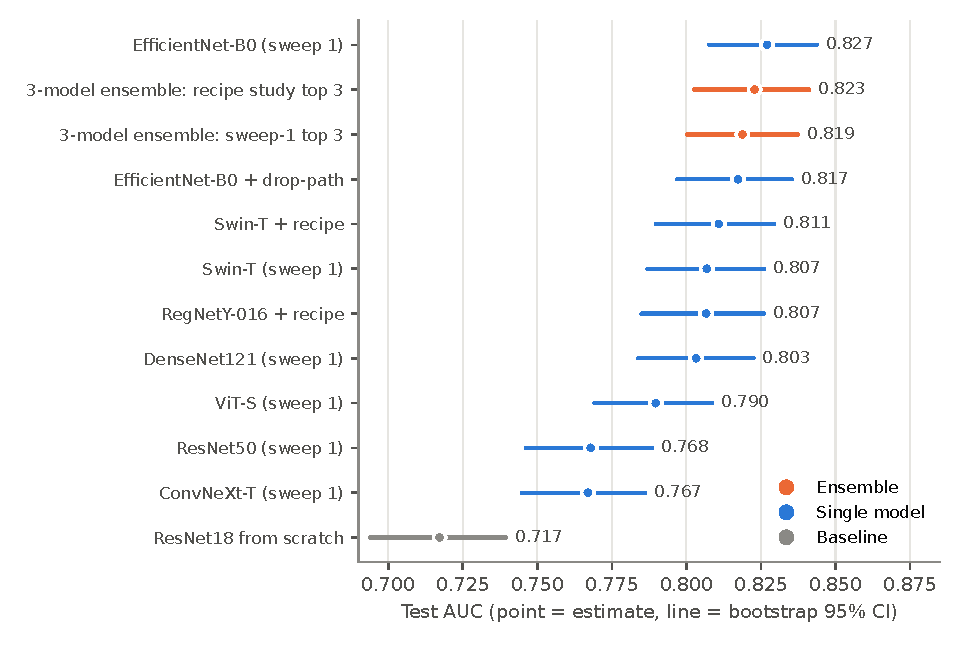
\includegraphics[width=0.82\linewidth]{figs/results_overview.pdf}
\caption{Test AUC with bootstrap 95\% confidence intervals for the main single models, the baseline, and the best ensembles. Sweep~1 = plain recipe; ``+ recipe'' = stronger recipe (Section~3.3).}
\label{fig:overview}
\end{figure}

\paragraph{Both modalities matter.}
With the same EfficientNet-B0 backbone, SLO alone gives 0.758 and OCT alone 0.764, while fusing both gives 0.827 (Figure~\ref{fig:modality}). Cross-domain transfer is poor:
a Swin-Tiny trained on SLO reaches 0.794 on SLO but only 0.677 on OCT, and the reverse gives 0.786 and 0.701 (Table~\ref{tab:sweep2}). The two images thus carry different information. Late fusion was slightly
better than early fusion for ResNet50 (0.768 vs 0.747, within the confidence intervals).

\begin{figure}[t]
\centering
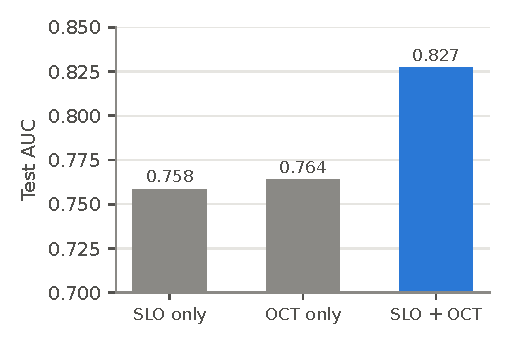
\includegraphics[width=0.48\linewidth]{figs/modality.pdf}
\caption{Contribution of each modality (EfficientNet-B0, first sweep).}
\label{fig:modality}
\end{figure}

\paragraph{Training recipe and what it taught us.}\label{sec:abl}
All models overfit strongly: the plain EfficientNet-B0 reaches training loss $\approx 0.008$ while validation AUC saturates early
(Figure~\ref{fig:overfit}). We therefore tried a stronger recipe (second and third sweeps). It did not help uniformly: Swin-Tiny was unchanged (0.808 $\pm$ 0.004 over three seeds, against 0.807 in sweep~1), but
EfficientNet-B0 \emph{dropped} from 0.827 to $0.798\pm0.003$ (three seeds, Table~\ref{tab:sweep3}).
We first suspected our EMA implementation, which copies batch-norm statistics from the live model instead of averaging them (a problem for batch-norm CNNs but not for the layer-norm Swin).
A single-factor ablation (Table~\ref{tab:abl}) \emph{refuted} this: switching EMA off lowered AUC further (0.786), so EMA helps. The main culprit was the
strong geometric augmentation: replacing rotation/scale/shift with flips and mild brightness jitter raised AUC from 0.798 to 0.819 ($\approx 7$ seed standard deviations), and a head learning rate of $1\times$ rather than $5\times$ gave a smaller gain (0.807).
A plausible reason (not tested) is that the images are spatially registered, so geometric transformations may destroy position-dependent cues, but we have no direct evidence.
Restoring all three choices (our approximate sweep-1 setup) gives 0.811, below the original 0.827, so some of the sweep-1 figure is probably favourable single-seed luck.
Of the other regularisers, drop-path 0.2 with dropout 0.5 helped (0.817 against 0.798), whereas mixup/CutMix (0.800), a lower learning rate (0.790) and a shorter schedule (0.777) did not (Table~\ref{tab:sweep3}).
The three ablations vary one factor each with one seed, and the 2{,}000-image test set limits resolution, so we treat the ordering of the effects as indicative. We did not run the combination of the helpful changes (flip-only augmentation, drop-path, head learning rate $1\times$).

\begin{figure}[t]
\centering
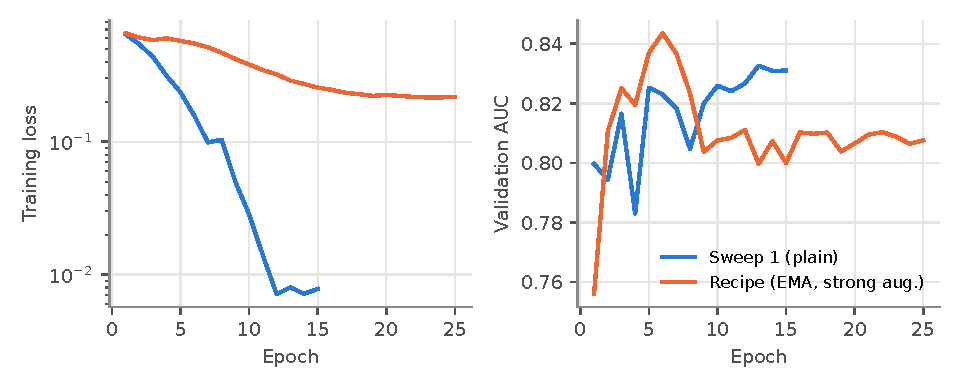
\includegraphics[width=0.85\linewidth]{figs/overfitting.pdf}
\caption{EfficientNet-B0: training loss (log scale) and validation AUC. The stronger recipe's loss stays higher because of label smoothing and augmentation, but its validation AUC peaks around epoch 6 and then declines.}
\label{fig:overfit}
\end{figure}

\begin{table}[t]
\centering\small
\resizebox{\linewidth}{!}{\begin{tabular}{lrrr}
\toprule
EfficientNet-B0 variant & Val AUC & Test AUC & TTA AUC \\
\midrule
Recipe (3 seeds, mean $\pm$ s.d.) & 0.832 & 0.798 $\pm$ 0.003 & 0.803 \\
\midrule
EMA off & 0.817 & 0.786 & 0.792 \\
Head LR $\times$1 (instead of $\times$5) & 0.828 & 0.807 & 0.807 \\
Flip + mild jitter only (no rotate/scale/shift) & 0.853 & 0.819 & 0.824 \\
All three reverted, no label smoothing, 15 epochs (approx. sweep-1 setup) & 0.844 & 0.811 & 0.814 \\
Sweep-1 run (original code, one seed) & 0.833 & 0.827 & 0.828 \\
\bottomrule
\end{tabular}
}
\caption{Single-factor ablations of the stronger recipe (EfficientNet-B0, one seed each; the recipe row is the three-seed mean). The last row is the original first-sweep run.}
\label{tab:abl}
\end{table}

\paragraph{Ensembling.}
Averaging models is the most consistent gain (Table~\ref{tab:ens}). The five-fold models score 0.789--0.808 individually (mean 0.800) and 0.830 together; the five diverse first-sweep models average 0.804 individually and reach 0.833 as an ensemble.
The best ensemble (five folds plus three train+validation models) reaches 0.834 [0.816, 0.852]. Flip TTA adds 0.001--0.010. Note that ensembles only match the best single first-sweep run (0.827) within uncertainty, so their advantage is mostly in not depending on one lucky run.
Training on all 3{,}000 images (no validation set) did not help single models (0.791--0.794); we used the final-epoch model there.

\begin{table}[t]
\centering\footnotesize
\setlength{\tabcolsep}{3pt}
\resizebox{\linewidth}{!}{\begin{tabular}{llrrrrr}
\toprule
Ensemble (average of probabilities) & $n$ & Members' mean AUC & Test AUC & 95\% CI & TTA AUC & ES-AUC race \\
\midrule
Top 3 of the recipe study by validation AUC & 3 & 0.806 & 0.823 & [0.803, 0.841] & 0.824 & 0.799 \\
Top 3 of sweep 1 by validation AUC (Swin-T, ViT-S, DenseNet121) & 3 & 0.800 & 0.819 & [0.800, 0.837] & 0.822 & 0.805 \\
3 seeds trained on train+val (EfficientNet-B0) & 3 & 0.792 & 0.816 & [0.797, 0.834] & 0.821 & 0.764 \\
\bottomrule
\end{tabular}
}
\caption{Probability-averaging ensembles. Members were chosen in advance or by validation AUC.}
\label{tab:ens}
\end{table}

\paragraph{Fairness.}
Performance is similar across gender and race groups (Table~\ref{tab:groups}): within-group AUCs differ by about 0.01--0.03 for most models, and ES-AUC for race is 0.75--0.82 (the highest, 0.821, for ensembles).
The Hispanic group (83 test images) shows the largest and least stable differences (AUC 0.74--0.81 across models), which sampling noise on so few images could explain.
The fairness-specific losses gave no consistent benefit (Table~\ref{tab:sweep2}, Swin-Tiny): the FIS-like loss and adversarial debiasing were within noise of the plain recipe (0.806 and 0.805 vs 0.808), and group reweighting was lower (0.787).
On EfficientNet-B0 the adversarial variant scored 0.802 against 0.817 for the config it extends (Table~\ref{tab:sweep3}). Adding age as an input did not help (0.808).
For reference, giving the model the visual-field mean deviation MD, a clinical measure closely tied to the label, raises AUC to 0.958, which shows how much of the label lives in that variable. We exclude it from every comparison.

\begin{table}[t]
\centering\footnotesize
\setlength{\tabcolsep}{4pt}
\resizebox{\linewidth}{!}{\begin{tabular}{lrrrrrrr}
\toprule
 & Female & Male & Asian & Black & White & Non-Hisp. & Hispanic \\
$n$ (test) & 1449 & 551 & 177 & 301 & 1522 & 1917 & 83 \\
\midrule
EfficientNet-B0 (sweep 1) & 0.824 & 0.835 & 0.823 & 0.816 & 0.827 & 0.830 & 0.740 \\
Swin-T + recipe (sweep 2) & 0.813 & 0.806 & 0.832 & 0.811 & 0.806 & 0.812 & 0.782 \\
EfficientNet-B0 + drop-path (sweep 3) & 0.816 & 0.822 & 0.831 & 0.803 & 0.814 & 0.819 & 0.811 \\
5-model ensemble (sweep 1) & 0.833 & 0.835 & 0.829 & 0.826 & 0.830 & 0.834 & 0.796 \\
8-model ensemble (sweep 3) & 0.832 & 0.841 & 0.856 & 0.821 & 0.829 & 0.836 & 0.806 \\
\bottomrule
\end{tabular}
}
\caption{Test AUC within demographic groups for representative models and ensembles.}
\label{tab:groups}
\end{table}

\paragraph{Cost.}
Single runs took from about 3 minutes (ResNet18) to 18 minutes (ConvNeXt-Tiny, 15 epochs) in sweep~1 and about 11--22 minutes in the later sweeps on the P100; EfficientNet-B0 was the cheapest of the strong models.

\subsection{Limitations}
(i)~The test set has 2{,}000 images, so confidence intervals are about $\pm0.02$; most differences in this report are within them.
(ii)~Most results are from a single seed. (iii)~Automatic selection used validation data only, but we did read test results while planning later sweeps, so the later configurations are not entirely free of test-set influence.
(iv)~The validation set (450 images) is itself noisy; Swin-Tiny had the best validation AUC in sweep~1 yet not the best test AUC.
(v)~Our FIS-like loss and ES-AUC are our own implementations. (vi)~We did not implement the published FIN/FIS/FIA methods or compare to published numbers, and our data may differ from the full 10{,}000-sample FairDomain release.

%==============================================================================
\section{Conclusions}
On this two-modality glaucoma classification task, the most important factors were \emph{using ImageNet-pretrained weights} (+0.03 to +0.11 AUC over a from-scratch baseline), \emph{using both modalities} (0.827 versus 0.758--0.764 for either alone), and
\emph{averaging several models} (about +0.03 over a typical member). The choice of architecture family, fairness-specific losses and most extra regularisers made no difference that we can distinguish from noise
on a 2{,}000-image test set. One recipe component, strong geometric augmentation, measurably hurt (about $-0.02$ AUC), and our hypothesis that EMA batch-norm statistics were responsible was wrong: EMA helped. All three
ablations were single runs, and the sweep-1 EfficientNet result (0.827) is probably optimistic. Fairness gaps across gender and race were small; the Hispanic group is too small to judge.

The strengths of our approach are its simplicity (standard pretrained backbones, two branches, probability averaging) and an evaluation that reports uncertainty and per-group results. Its weaknesses are the small data scale, limited seeds, and the absence of the published fairness methods for comparison.

\paragraph{Future work.}
(1)~Combine the helpful changes (flip-only augmentation, drop-path, head learning rate $1\times$, EMA) and test them with several seeds. (2)~Implement FIN, FIS and FIA faithfully and compare on the full dataset, and extend to the segmentation
task if masks are available. (3)~Fine-tune retinal foundation models. (4)~Use the two image types as source and target domains with domain-adaptation methods, since transfer between them is poor.
(5)~Use cross-validation over train and test to reduce the noise from a single 2{,}000-image test split.

%==============================================================================
\begin{thebibliography}{99}\small
\bibitem{fairdomain} Y.~Tian, C.~Wen, M.~Shi, M.~M.~Afzal, H.~Huang, M.~O.~Khan, Y.~Luo, Y.~Fang, and M.~Wang. FairDomain: Achieving fairness in cross-domain medical image segmentation and classification. In \emph{ECCV}, 2024. arXiv:2407.08813.
\bibitem{harvardgf} Y.~Luo et al. Harvard Glaucoma Fairness: A retinal nerve disease dataset for fairness learning and fair identity normalization. \emph{IEEE Trans.\ Medical Imaging}. arXiv:2306.09264.
\bibitem{harvardeye} Y.~Luo, Y.~Tian, M.~Shi, T.~Elze, and M.~Wang. Harvard Eye Fairness: A large-scale 3D imaging dataset for equitable eye diseases screening and fair identity scaling. arXiv:2310.02492, 2023.
\bibitem{fairclip} Y.~Luo et al. FairCLIP: Harnessing fairness in vision-language learning. In \emph{CVPR}, 2024. arXiv:2403.19949.
\bibitem{fairenc} FairEnc: A fair vision-language model with fair vision and text encoders for glaucoma detection. arXiv:2605.04882.
\bibitem{faireyenet} Fair-Eye Net: A fair, trustworthy, multimodal integrated glaucoma full chain AI system. arXiv:2601.18464.
\bibitem{redsphere} RED-Sphere: Hyperspherical residual edge debiasing for cross-population fundus disease domain generalization. arXiv:2607.10777.
\bibitem{resnet} K.~He, X.~Zhang, S.~Ren, and J.~Sun. Deep residual learning for image recognition. In \emph{CVPR}, 2016.
\bibitem{efficientnet} M.~Tan and Q.~V.~Le. EfficientNet: Rethinking model scaling for convolutional neural networks. In \emph{ICML}, 2019.
\bibitem{densenet} G.~Huang, Z.~Liu, L.~van der Maaten, and K.~Q.~Weinberger. Densely connected convolutional networks. In \emph{CVPR}, 2017.
\bibitem{regnet} I.~Radosavovic, R.~P.~Kosaraju, R.~Girshick, K.~He, and P.~Doll\'ar. Designing network design spaces. In \emph{CVPR}, 2020.
\bibitem{convnext} Z.~Liu, H.~Mao, C.-Y.~Wu, C.~Feichtenhofer, T.~Darrell, and S.~Xie. A ConvNet for the 2020s. In \emph{CVPR}, 2022.
\bibitem{vit} A.~Dosovitskiy et al. An image is worth 16x16 words: Transformers for image recognition at scale. In \emph{ICLR}, 2021.
\bibitem{deit} H.~Touvron, M.~Cord, M.~Douze, F.~Massa, A.~Sablayrolles, and H.~J\'egou. Training data-efficient image transformers and distillation through attention. In \emph{ICML}, 2021.
\bibitem{swin} Z.~Liu, Y.~Lin, Y.~Cao, H.~Hu, Y.~Wei, Z.~Zhang, S.~Lin, and B.~Guo. Swin Transformer: Hierarchical vision transformer using shifted windows. In \emph{ICCV}, 2021.
\bibitem{coatnet} Z.~Dai, H.~Liu, Q.~V.~Le, and M.~Tan. CoAtNet: Marrying convolution and attention for all data sizes. In \emph{NeurIPS}, 2021.
\bibitem{maxvit} Z.~Tu, H.~Talebi, H.~Zhang, F.~Yang, P.~Milanfar, A.~Bovik, and Y.~Li. MaxViT: Multi-axis vision transformer. In \emph{ECCV}, 2022.
\bibitem{dinov2} M.~Oquab et al. DINOv2: Learning robust visual features without supervision. \emph{Transactions on Machine Learning Research}, 2024.
\bibitem{imagenet} O.~Russakovsky et al. ImageNet large scale visual recognition challenge. \emph{IJCV}, 2015.
\bibitem{timm} R.~Wightman. PyTorch Image Models (timm). \url{https://github.com/huggingface/pytorch-image-models}, 2019.
\bibitem{pytorch} A.~Paszke et al. PyTorch: An imperative style, high-performance deep learning library. In \emph{NeurIPS}, 2019.
\bibitem{adamw} I.~Loshchilov and F.~Hutter. Decoupled weight decay regularization. In \emph{ICLR}, 2019.
\bibitem{onecycle} L.~N.~Smith and N.~Topin. Super-convergence: Very fast training of neural networks using large learning rates. In \emph{Artificial Intelligence and Machine Learning for Multi-Domain Operations Applications}, SPIE, 2019.
\bibitem{mixup} H.~Zhang, M.~Cisse, Y.~N.~Dauphin, and D.~Lopez-Paz. mixup: Beyond empirical risk minimization. In \emph{ICLR}, 2018.
\bibitem{cutmix} S.~Yun, D.~Han, S.~J.~Oh, S.~Chun, J.~Choe, and Y.~Yoo. CutMix: Regularization strategy to train strong classifiers with localizable features. In \emph{ICCV}, 2019.
\bibitem{stochdepth} G.~Huang, Y.~Sun, Z.~Liu, D.~Sedra, and K.~Q.~Weinberger. Deep networks with stochastic depth. In \emph{ECCV}, 2016.
\bibitem{labelsmooth} C.~Szegedy, V.~Vanhoucke, S.~Ioffe, J.~Shlens, and Z.~Wojna. Rethinking the Inception architecture for computer vision. In \emph{CVPR}, 2016.
\bibitem{grl} Y.~Ganin and V.~Lempitsky. Unsupervised domain adaptation by backpropagation. In \emph{ICML}, 2015.
\end{thebibliography}

%==============================================================================
\appendix
\section{Full results of each sweep}
\begin{table}[h]
\centering\footnotesize
\setlength{\tabcolsep}{3pt}
\resizebox{\linewidth}{!}{\begin{tabular}{llrrrrrr}
\toprule
Model & Type & Params (M) & Val AUC & Test AUC & TTA AUC & Acc. & Worst-group AUC \\
\midrule
EfficientNet-B0 & CNN & 8.0 & 0.833 & 0.827 & 0.828 & 0.763 & 0.816 \\
Swin-Tiny & Transformer & 55.0 & 0.844 & 0.807 & 0.811 & 0.739 & 0.796 \\
DenseNet121 & CNN & 13.9 & 0.837 & 0.803 & 0.810 & 0.740 & 0.794 \\
CoAtNet-0 & Hybrid & 53.3 & 0.835 & 0.793 & 0.796 & 0.716 & 0.787 \\
ViT-Small & Transformer & 42.9 & 0.841 & 0.790 & 0.792 & 0.724 & 0.781 \\
MaxViT-Tiny (early fusion) & Hybrid & 28.6 & 0.820 & 0.778 & 0.788 & 0.715 & 0.768 \\
DeiT-Small (early fusion) & Transformer & 21.6 & 0.812 & 0.768 & 0.774 & 0.706 & 0.756 \\
ResNet50 & CNN & 47.0 & 0.796 & 0.768 & 0.779 & 0.703 & 0.741 \\
ConvNeXt-Tiny & CNN & 55.6 & 0.822 & 0.767 & 0.767 & 0.680 & 0.757 \\
EfficientNet-B0, OCT only & Single modality & 4.0 & 0.809 & 0.764 & 0.771 & 0.683 & 0.753 \\
EfficientNet-B0, SLO only & Single modality & 4.0 & 0.806 & 0.758 & 0.762 & 0.673 & 0.723 \\
ResNet50 (early fusion) & CNN & 23.5 & 0.746 & 0.747 & 0.759 & 0.688 & 0.745 \\
ResNet18 (scratch) & CNN & 22.3 & 0.773 & 0.717 & 0.725 & 0.666 & 0.706 \\
\bottomrule
\end{tabular}
}
\caption{Sweep 1: 13 configurations, plain recipe, 15 epochs, validation-based epoch selection. Params = total parameters of both branches. ``TTA AUC'' = with horizontal-flip test-time averaging.}
\label{tab:sweep1}
\end{table}

\begin{table}[h]
\centering\footnotesize
\setlength{\tabcolsep}{3pt}
\resizebox{\linewidth}{!}{\begin{tabular}{lrrrrrr}
\toprule
Variant (Swin-Tiny backbone) & Val AUC & Test AUC & 95\% CI & ES-AUC race & Worst-group & Other-domain AUC \\
\midrule
+ age and MD (upper bound) & 0.963 & 0.958 & [0.950, 0.965] & 0.938 & 0.941 & -- \\
Gated fusion + modality dropout & 0.842 & 0.812 & [0.793, 0.832] & 0.800 & 0.803 & -- \\
Swin-T + recipe & 0.834 & 0.811 & [0.790, 0.831] & 0.790 & 0.806 & -- \\
Swin-T + recipe (seed 2) & 0.836 & 0.810 & [0.789, 0.830] & 0.783 & 0.793 & -- \\
DINOv2-S fine-tune & 0.837 & 0.809 & [0.788, 0.829] & 0.760 & 0.786 & -- \\
+ age as input & 0.840 & 0.808 & [0.786, 0.828] & 0.785 & 0.802 & -- \\
FIS-like loss & 0.847 & 0.806 & [0.784, 0.826] & 0.779 & 0.800 & -- \\
Adversarial race debiasing & 0.850 & 0.805 & [0.782, 0.823] & 0.788 & 0.801 & -- \\
Swin-T + recipe (seed 1) & 0.843 & 0.803 & [0.782, 0.823] & 0.783 & 0.797 & -- \\
ViT-S cross-attention fusion & 0.844 & 0.795 & [0.773, 0.815] & 0.772 & 0.786 & -- \\
Train SLO $\to$ test OCT & 0.796 & 0.794 & [0.773, 0.812] & 0.759 & 0.786 & 0.677 \\
Group-reweighted loss & 0.819 & 0.787 & [0.764, 0.808] & 0.760 & 0.780 & -- \\
Train OCT $\to$ test SLO & 0.822 & 0.786 & [0.765, 0.804] & 0.758 & 0.779 & 0.701 \\
\bottomrule
\end{tabular}
}
\caption{Sweep 2: stronger recipe on Swin-Tiny (the backbone with the best validation AUC in sweep 1), 25 epochs. The ``+ age and MD'' row is an upper bound and not a fair comparison.}
\label{tab:sweep2}
\end{table}

\begin{table}[h]
\centering\footnotesize
\setlength{\tabcolsep}{3pt}
\resizebox{\linewidth}{!}{\begin{tabular}{lrrrrrr}
\toprule
Configuration & Val AUC & Test AUC & 95\% CI & TTA AUC & ES-AUC race & Worst-group \\
\midrule
EfficientNet-B0 + recipe & 0.844 & 0.799 & [0.779, 0.820] & 0.802 & 0.774 & 0.782 \\
\quad seed 1 & 0.818 & 0.795 & [0.774, 0.815] & 0.801 & 0.747 & 0.782 \\
\quad seed 2 & 0.835 & 0.800 & [0.778, 0.821] & 0.805 & 0.755 & 0.777 \\
\quad 12 epochs & 0.836 & 0.777 & [0.757, 0.798] & 0.787 & 0.760 & 0.766 \\
\quad + mixup/CutMix & 0.839 & 0.800 & [0.780, 0.819] & 0.805 & 0.765 & 0.786 \\
\quad + drop-path 0.2, dropout 0.5 & 0.852 & 0.817 & [0.797, 0.839] & 0.820 & 0.793 & 0.803 \\
\quad lower LR (2e-4) & 0.833 & 0.790 & [0.767, 0.812] & 0.803 & 0.779 & 0.783 \\
\quad gated fusion + modality dropout & 0.832 & 0.810 & [0.791, 0.830] & 0.814 & 0.801 & 0.803 \\
\midrule
EfficientNet-B2 & 0.839 & 0.796 & [0.778, 0.817] & 0.806 & 0.765 & 0.783 \\
EfficientNet-B3 & 0.821 & 0.779 & [0.759, 0.799] & 0.789 & 0.738 & 0.757 \\
RegNetY-016 & 0.831 & 0.807 & [0.785, 0.828] & 0.812 & 0.773 & 0.803 \\
DenseNet121 & 0.828 & 0.781 & [0.760, 0.801] & 0.791 & 0.739 & 0.768 \\
\midrule
Drop-path config + adversarial race debiasing & 0.847 & 0.802 & [0.781, 0.821] & 0.807 & 0.782 & 0.796 \\
\bottomrule
\end{tabular}
}
\caption{Sweep 3: EfficientNet-B0 regularisation and backbone neighbours, 25 epochs unless stated. The drop-path configuration had the best validation AUC (0.852) and was used for the 5-fold and train+validation runs.}
\label{tab:sweep3}
\end{table}

\end{document}
